\documentclass[tikz,border=2]{standalone}
\usetikzlibrary{shadows,arrows,shapes,positioning,calc,backgrounds,fit}
% Define the layers to draw the diagram
%
\begin{document}
\pgfdeclarelayer{bg}
\pgfdeclarelayer{fg}
\pgfsetlayers{bg,main,fg}
%
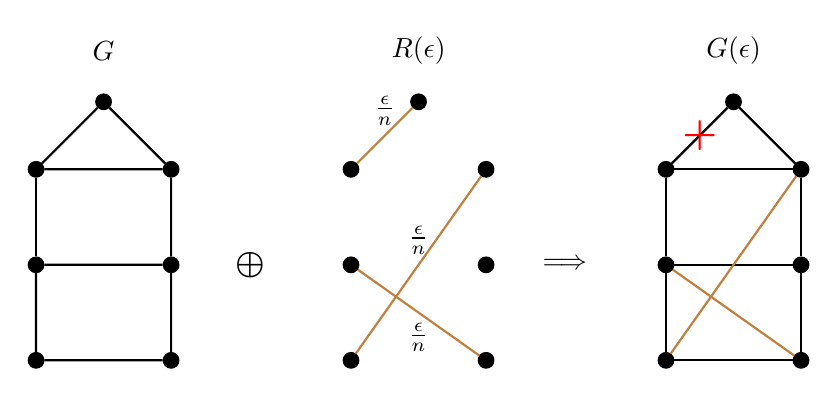
\begin{tikzpicture}
[node distance=1cm,
vertex/.style={shape=circle,draw=black,inner sep=2pt},
infected/.style={vertex,fill=red},
uninfected/.style={vertex,fill=black},
myedge/.style={thick},
randedge/.style={thick,color=brown},
dedge/.style={>=latex', shorten >=.0pt, shorten <=.0pt, thick},
infedge/.style={line width=3,color=white!75!black}]

\node (v1) [uninfected] at (0,0) {};
\node (v2) [uninfected,below left=of v1] {};
\node (v3) [uninfected,below right=of v1] {};
\node (v4) [uninfected,below=of v2] {};
\node (v5) [uninfected,below=of v3] {};
\node (v6) [uninfected,below=of v4] {};
\node (v7) [uninfected,below=of v5] {};
\draw[myedge] (v1) -- (v2) -- (v3) -- (v5) -- (v4) -- (v6) -- (v7)
-- (v5);
\draw[myedge] (v1) -- (v3);
\draw[myedge] (v2) -- (v4);
\node [above of=v1,yshift=-10] {$G$};
\node [right of=v5] {\large{\boldmath $\oplus$}};

\node (v1) [uninfected] at (4,0) {};
\node (v2) [uninfected,below left=of v1] {};
\node (v3) [uninfected,below right=of v1] {};
\node (v4) [uninfected,below=of v2] {};
\node (v5) [uninfected,below=of v3] {};
\node (v6) [uninfected,below=of v4] {};
\node (v7) [uninfected,below=of v5] {};
\draw[randedge] (v1) -- (v2) node[midway,above,color=black] {$\frac{\epsilon}{n}$};
\draw[randedge] (v4) -- (v7) node[midway,below,color=black] {$\frac{\epsilon}{n}$};
\draw[randedge] (v3) -- (v6) node[midway,above,color=black] {$\frac{\epsilon}{n}$};
\node [above of=v1,yshift=-10] {$R(\epsilon)$};
\node [right of=v5] {$\Longrightarrow$};

\node (v1) [uninfected] at (8,0) {};
\node (v2) [uninfected,below left=of v1] {};
\node (v3) [uninfected,below right=of v1] {};
\node (v4) [uninfected,below=of v2] {};
\node (v5) [uninfected,below=of v3] {};
\node (v6) [uninfected,below=of v4] {};
\node (v7) [uninfected,below=of v5] {};
\draw[myedge] (v2) -- (v3) -- (v5) -- (v4) -- (v6) -- (v7)
-- (v5);
\draw[myedge] (v1) -- (v3);
\draw[myedge] (v2) -- (v4);
\draw[randedge] (v4) -- (v7);
\draw[randedge] (v3) -- (v6);
\draw[myedge] (v2) -- (v1) node[midway,color=red] {\Large{\boldmath $+$}};
\node [above of=v1,yshift=-10] {$G(\epsilon)$};
%\begin{pgfonlayer}{bg}
%\draw[infedge] (v2) -- (v1);
%\end{pgfonlayer}

\end{tikzpicture}
{}
\end{document}
